\documentclass{article}

\usepackage[]{../.template/xrcise}

\subject{Natural Language Processing}
\semester{Winter 2024}
\author{Leopold Lemmermann}

\begin{document}\createtitle

\sheet{Quizzes}

\begin{exercise}{Quiz I}
  \begin{enumerate}
    \item What are three examples of NLP applications on the web?
    \item How can the web improve the quality of NLP? List three examples.
    \item What two types of segments are important in NLP pipelines?
  \end{enumerate}

  \begin{solution}
    \begin{enumerate}
      \item Internet of Services, Community mining, Information retrieval, ...
      \item Web as Corpus, Analyzing web-based knowledge repositories, ...
      \item Sentence, Token.
    \end{enumerate}
  \end{solution}
\end{exercise}

\begin{exercise}{Quiz II}
  \begin{enumerate}
    \item Identify all stems and affixes in the following words: "index," "incorrect," "interesting."
    \item In contrast to lemmatization, stemming does not necessarily return a valid word form. Why is stemming still useful?
    \item What types of syntactic ambiguity do you know? List at least two types with an example for each type.
  \end{enumerate}

  \begin{solution}
    \begin{enumerate}
      \item \begin{itemize}
          \item \textbf{index}: stem = "index"
          \item \textbf{incorrect}: prefix = "in," stem = "correct"
          \item \textbf{interesting}: stem = "interest," suffix = "ing"
        \end{itemize}
      \item Faster, easier, applications in IR.
      \item Attachment ambiguity (e.g. "He walked around the house with the dog."), coordination ambiguity (e.g. "We serve excellent rice and fish."), garden path sentences (e.g. "The loud shot the silent.").
    \end{enumerate}
  \end{solution}
\end{exercise}

\begin{exercise}{Quiz III}
  \begin{enumerate}
    \item Why are more features not always better for learning a classifier?
    \item What is the typical type of input data that a sequence tagger training step requires?
  \end{enumerate}

  \begin{solution}
    \begin{enumerate}
      \item More training data might be needed; Dependent features might lead to deficient models; Some ML algorithms can only deal with specific data types; Slower.
      \item Labeled training text. (e.g. POS, NER)
    \end{enumerate}
  \end{solution}
\end{exercise}

\begin{exercise}{Quiz IV}
  \begin{enumerate}
    \item What is the correct order of tasks in a web search engine: crawling, parsing, stemming, indexing, ranking?
    \item Name features and their types used for WebSearch ranking.
    \item Why not use user clicks for ranking after having a few million clicks from a previously unranked search engine?
  \end{enumerate}

  \begin{solution}
    \begin{enumerate}
      \item Crawling, parsing, stemming, indexing, ranking.
      \item Static features: inlinks, pagerank, document length, language quality. Dynamic features: TF-IDF, LM scores, anchor text, user clicks. Query features: length, known bigrams, number of stopwords.
      \item Top-result-bias.
    \end{enumerate}
  \end{solution}
\end{exercise}

\begin{exercise}{Quiz V}
  \begin{enumerate}
    \item Relate the following queries to query types: "facebook," "NSA scandal," "facebook alternatives," "facebook data migration tool."
    \item What is the difference between extrinsic and intrinsic evaluation?
  \end{enumerate}

  \begin{solution}
    \begin{enumerate}
      \item facebook: navigational, NSA scandal: informational, facebook alternatives: exploratory, facebook data migration tool: transactional.
      \item Intrinsic evaluation measures the performance of a specific component or model, while extrinsic evaluation assesses the impact of improvements on larger tasks or systems.
    \end{enumerate}
  \end{solution}
\end{exercise}

\begin{exercise}{Quiz VI}
  \begin{enumerate}
    \item The trigram language model generates the following word based on three previous words.
    \item A 7-gram model generally performs worse than a 5-gram model because there is not enough training data to estimate its parameters well.
    \item The trigram language model generates syntactically correct sentences.
    \item With the trigram language model, all words are always equally probable.
    \item A generative language model always provides the same output for the same input.
    \item Language models can only perform tasks for which they have been trained directly with examples.
    \item Training dialog-based language models such as chatGPT requires a lot of human feedback in addition to large amounts of text.
  \end{enumerate}

  \begin{solution}
    \begin{enumerate}
      \item False
      \item True
      \item False
      \item False
      \item False
      \item False
      \item True
    \end{enumerate}
  \end{solution}
\end{exercise}

\begin{exercise}{Quiz VII}
  Assign the procedures for defining/teaching tasks to LLMs to the definitions:
  \begin{enumerate}
    \item\label{ex:assign-1} tasks are explained directly in the prompt
    \item\label{ex:assign-2}  a smaller model is trained using training data created from a larger model
    \item\label{ex:assign-3}  tasks are explained in the prompt using several examples
    \item\label{ex:assign-4}  the model is trained further with the help of manually created training data
  \end{enumerate}
  \begin{enumerate}
    \item\label{ex:assign-a}  Few-Shot
    \item\label{ex:assign-b}  Zero-Shot
    \item\label{ex:assign-c}  Model distillation
    \item\label{ex:assign-d}  Fine-tuning
  \end{enumerate}

  \begin{solution}
    \begin{enumerate}
      \item\ref{ex:assign-1} $\to$ \ref{ex:assign-b}
      \item\ref{ex:assign-2} $\to$ \ref{ex:assign-c}
      \item\ref{ex:assign-3} $\to$ \ref{ex:assign-a}
      \item\ref{ex:assign-4} $\to$ \ref{ex:assign-d}
    \end{enumerate}
  \end{solution}
\end{exercise}

\begin{exercise}{Quiz VIII}
  \begin{enumerate}
    \item List three different question types with an example for each of them.
    \item Give a schema on how these Question Answering System components interact: Answer, Document processing, Document collection, Answer processing, Question, Question processing.
  \end{enumerate}

  \begin{solution}
    \begin{enumerate}
      \item \begin{itemize}
          \item \textbf{Feature specification}: What shape did the stone have?
          \item \textbf{Definition}: What are prime numbers?
          \item \textbf{Quantification}: How many Bavarians required for exchanging a light bulb?
        \end{itemize}
      \item Query Formulation, Query Classificatio, Indexing, Document Retrieval, Passage Retrieval
        \begin{figure}
  \center
  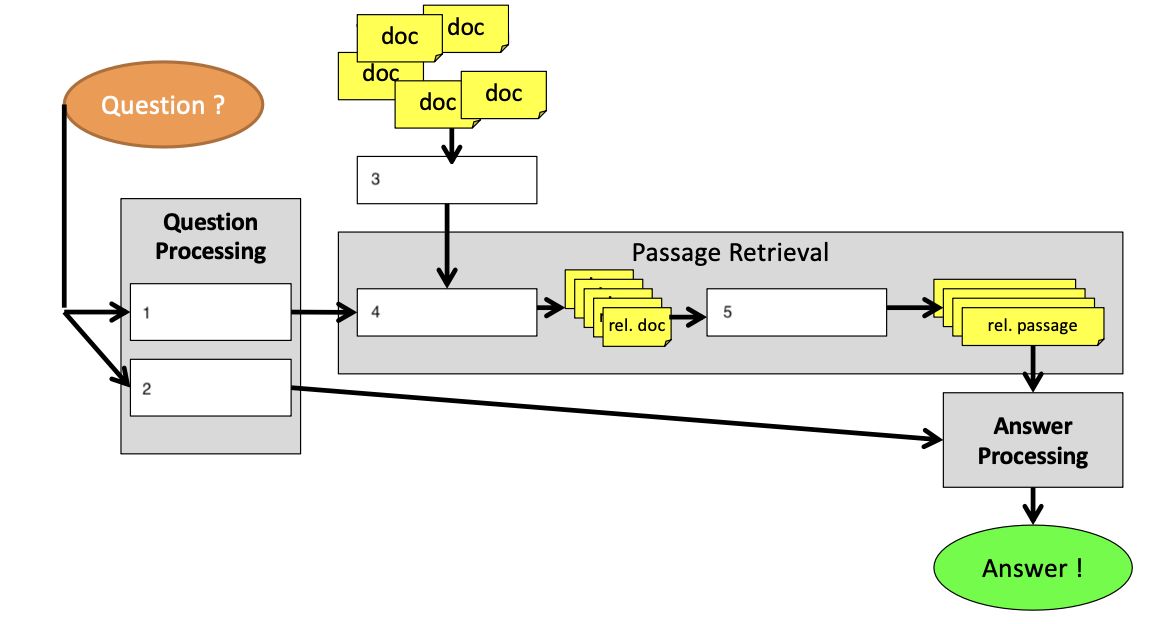
\includegraphics[width=.8\textwidth]{res/qa.png}
  \caption{Question Answering}\label{fig:qa}
\end{figure}
    \end{enumerate}
  \end{solution}
\end{exercise}

\begin{exercise}{Quiz IX}
  The Reciprocal Rank (RR) is the inverse of the rank of the first correct answer or 0 if no correct answer was given. The Mean Reciprocal Rank (MRR) is the mean of the RRs over all questions. P@1 is the precision on the first result. Which measure is more suited for question answering, and why?

  \begin{solution}
    In question answering, the goal is to retrieve the correct answer to a question. Therefore, the precision of the first result (P@1) is more suited for evaluating QA systems. MRR is better suited for information retrieval tasks where multiple relevant documents may exist.
  \end{solution}
\end{exercise}

\begin{exercise}{Quiz X}
  \begin{enumerate}
    \item What are the limits of sentiment analysis based on word lists?
    \item What is counterspeech, and what is needed to build a system that performs counterspeech?
  \end{enumerate}

  \begin{solution}
    \begin{enumerate}
      \item Meaning is context-dependent (e.g., "small" can be good or bad), sentiment is expressed implicitly, statements can be negated (e.g., "not good"), and word lists are always incomplete.
      \item Counterspeech is speaking up against abusive, harmful, hate content. To build a system, one needs a detector of abusive content and a generative language model to explain why the content is hateful and why it is unwanted. This requires training data for detection (easy) and counterspeech (hard, rare).
    \end{enumerate}
  \end{solution}
\end{exercise}



\sheet[2023]{Exam}

\begin{exercise}{Tokenization ambiguity}\label{ex:tokenization}
  List three types of tokenization ambiguity and explain each.

  \begin{solution}
    \begin{itemize}
      \item \textbf{Hyphenation}: Is "state-of-the-art" one token or three?
      \item \textbf{Punctuation}: Should periods in abbreviations (e.g., "U.S.") be separated?
      \item \textbf{Contractions}: Should "don't" be split into "do" and "n't"?
      \item \textbf{Language differences}: Tokenization rules vary by language (e.g., Chinese characters vs. English words).
    \end{itemize}
  \end{solution}
\end{exercise}

\begin{exercise}{Parsing ambiguity}
  \begin{quote}\center "\textit{John shot the man with the gun}"\end{quote}
  Draw all possible parse trees for this sentence using the English grammar. What types of syntactic ambiguity are present?

  \begin{solution}
    A parse tree can be drawn using the following structures: $S, N, V, Det, P, NP, VP, PP$. This is an example of attachment ambiguity. The prepositional phrase "with the gun" can attach to either "shot" or "the man".
  \end{solution}
\end{exercise}

\begin{exercise}{Stemming v. Lemmatization}\label{ex:stem-v-lemm}
  \begin{enumerate}
    \item What is the difference between stemming and lemmatization?
    \item In contrast to lemmatization, stemming does not necessarily return a valid word form. Why is stemming still useful?
    \item Identify all stems and affixes (prefix, suffix, infix, circumfix) in the following words: "index," "incorrect," "interesting."
  \end{enumerate}

  \begin{solution}
    \begin{enumerate}
        \item Stemming reduces words to their root form by removing affixes. Lemmatization finds the base or dictionary form of a word based on its context.
        \item Stemming is useful for information retrieval tasks where speed is crucial, and minor inaccuracies are acceptable.
        \item \begin{itemize}
            \item \textbf{index}: stem = "index"
            \item \textbf{incorrect}: prefix = "in," stem = "correct"
            \item \textbf{interesting}: stem = "interest," suffix = "ing"
        \end{itemize}
    \end{enumerate}
  \end{solution}
\end{exercise}

\begin{exercise}{Machine learning}\label{ex:ml}
  \begin{enumerate}
    \item Which of the following statements are correct? Give a brief explanation for each.
      \begin{itemize}
        \item[$\square$] Features for Naive Bayes classifiers do not need to be uncorrelated.
        \item[$\square$] Naive Bayes is slow to train.
        \item[$\square$] SVM itself is a multi-label classifier.
        \item[$\square$] SVM handles sparse data well.
      \end{itemize}
      \item Explain Support Vector Machines when you have more than two classes.
      \item What are the main stages in a machine learning pipeline?
  \end{enumerate}

  \begin{solution}
    \begin{enumerate}
      \item \begin{itemize}
          \item \textbf{True}: Features for Naive Bayes do not need to be uncorrelated, though it assumes independence for computation.
          \item \textbf{False}: Naive Bayes is fast to train, not slow.
          \item \textbf{False}: SVM is not inherently multi-label but can be adapted for multi-label classification.
          \item \textbf{True}: SVM handles sparse data well due to its kernel functions.
        \end{itemize}
      \item \begin{itemize}
          \item \textbf{One-vs-One (OvO)}: Trains a classifier for every pair of classes. Final classification is determined by majority voting.
          \item \textbf{One-vs-All (OvA)}: Trains one classifier per class against all other classes. The highest-confidence prediction is chosen.
        \end{itemize}
      \item Data Preprocessing $\to$ Feature extraction $\to$ Model training $\to$ Evaluation $\to$ Deployment
    \end{enumerate}
  \end{solution}
\end{exercise}

\begin{exercise}{Information retrieval}\label{ex:ir}
  Information retrieval (IR) is concerned with finding relevant information in large collections of data.
  \begin{enumerate}
    \item Describe stages in the IR cycle.
    \item Where is classification used in IR?
    \item What are key differences between Question Answering (QA) and IR?
  \end{enumerate}

  \begin{solution}
    \begin{enumerate}
        \item \begin{itemize}
            \item \textbf{Indexing}: Process and store data for efficient retrieval.
            \item \textbf{Querying}: Users submit queries to search the index.
            \item \textbf{Retrieval}: Return ranked results based on relevance scores.
            \item \textbf{Evaluation}: Assess performance using metrics like precision and recall.
          \end{itemize}
        \item In query classification, document classification, and relevance classification.
        \item QA provides direct answers, requires natural language understanding, and is used in chatbots. IR retrieves documents, focuses on keyword matching, and powers search engines.
    \end{enumerate}
  \end{solution}
\end{exercise}

\begin{exercise}{Corpus construction}\label{ex:corpus}
  \begin{enumerate}
    \item Define a corpus in the context of NLP.
    \item How would you construct a corpus usable for linguistic purposes?
  \end{enumerate}

  \begin{solution}
    \begin{enumerate}
      \item A corpus is a large collection of text data used for linguistic analysis, machine learning, or NLP research.
      \item \begin{enumerate}
          \item \textbf{Data collection}: Gather data from relevant sources (e.g., web crawling, domain-specific text).
          \item \textbf{Cleaning and preprocessing}: Remove duplicates, non-linguistic content, and normalize text (e.g., case normalization, tokenization).
          \item \textbf{Annotation}: Add metadata or linguistic labels (e.g., POS tags, syntactic trees) to the text.
          \item \textbf{Storage}: Store the corpus in an accessible format like JSON, XML, or relational databases.
          \item \textbf{Documentation}: Provide guidelines and metadata about the corpus for user understanding.
        \end{enumerate}
    \end{enumerate}
  \end{solution}
\end{exercise}

\begin{exercise}{Hate speech}\label{ex:hate-speech}
  \begin{enumerate}
    \item Define hate speech.
    \item How would you construct a hate speech classifier?
    \item Explain how to counter hate speech.
  \end{enumerate}

  \begin{solution}
    \begin{enumerate}
        \item Language that attacks or discriminates against individuals or groups based on attributes.
        \item Collect labeled datasets, preprocess text, extract features, train a model, and evaluate it.
        \item Collect examples of effective counter hate responses, classify hate speech, and generate counter-responses using NLP techniques.
    \end{enumerate}
  \end{solution}
\end{exercise}

\begin{exercise}{Crowdsourcing}\label{ex:crowdsourcing}
  \begin{enumerate}
    \item What is the workflow for crowdsourced annotation?
    \item What are opportunities and challenges in using crowdsourcing for data annotation?
  \end{enumerate}

  \begin{solution}
    \begin{enumerate}
        \item \textbf{Task design}: Define the annotation task clearly with examples and instructions.
        \item \textbf{Platform setup}: Use a crowdsourcing platform (e.g., Amazon Mechanical Turk, Prolific).
        \item \textbf{Quality control}: Include test questions and redundancy (multiple annotators per item) to ensure data reliability.
        \item \textbf{Data aggregation}: Aggregate annotations using majority voting or weighted schemes.
        \item \textbf{Evaluation}: Analyze annotation quality and address inconsistencies.
    \end{enumerate}
    \begin{itemize}
        \item[+] Fast and scalable data annotation.
        \item[+] Access to diverse annotators.
        \item[+] Cost-effective compared to hiring experts.
        \item[-] Quality control is challenging.
        \item[-] May introduce noise or bias.
        \item[-] Difficult to ensure annotator expertise.
    \end{itemize}
  \end{solution}
\end{exercise}

\begin{exercise}{Web as corpus}\label{ex:web-corpus}
  In NLP research, the web is often used as a corpus.
  \begin{enumerate}
    \item What are some opportunities of using the web as a corpus?
    \item The web contains many duplicates. How can they be detected?
    \item Explain other key challenges in using the web as a corpus.
  \end{enumerate}

  \begin{solution}
    \begin{enumerate}
      \item Large-scale, diverse data sources; up-to-date content; covers multiple languages and domains.
      \item Hashing (e.g., MD5, SHA) to compare file contents; cosine similarity or Jaccard index for text comparisons; comparing HTML structure or metadata.
      \item \begin{itemize}
          \item \textbf{Noise}: Content may contain errors, irrelevant information, or non-standard grammar.
          \item \textbf{Duplicates}: Identical or nearly identical data appears multiple times.
          \item \textbf{Bias}: Web content often reflects societal biases, which can skew analyses.
          \item \textbf{Reproducibility}: Web pages change frequently, making reproducibility challenging.
        \end{itemize}
    \end{enumerate}
  \end{solution}
\end{exercise}

\begin{exercise}{Classification metrics}\label{ex:class-metrics}
  Have a look at the classification results in Table \ref{tbl:results}. \begin{table}
  \center
  \begin{tabular}{c|cc|c}
    Actual/Predicted& \textbf{+} & \textbf{-} & \\ \hline
    \textbf{+} & 10 & 5 & 15 \\
    \textbf{-} & 3 & 12 & 15 \\ \hline
    & 13 & 17 & \textbf{30} \\
  \end{tabular}
  \caption{Experimental resulsts}\label{tbl:results}
\end{table}

  \begin{enumerate}
    \item Calculate Precision, Recall, and F1-Score. What is the problem with these metrics in IR?
    \item Calculate Cohen's Kappa. Why is it better for evaluating IR systems?
  \end{enumerate}
    
  \begin{solution}
    \begin{enumerate}
      \item \begin{itemize}
        \item \textbf{Precision} $\frac{TP}{TP + FP} = \frac{10}{10+5} = .6666$
        \item \textbf{Recall}: $\frac{TP}{TP + FN} = \frac{10}{10+3} = .7692$
        \item \textbf{F1-Score}: $2 \times \frac{\text{Precision} \times \text{Recall}}{\text{Precision} + \text{Recall}} = 2 \times \frac{.6666 \times .7692}{.6666 + .7692} = .7142$
        \end{itemize}
        These metrics are limited as they do not account for chance agreement.
      \item Cohen's Kappa is calculated as $\kappa = \frac{P_o - P_e}{1 - P_e}$ and describes the observed agreement $P_o$ relative to the expected agreement $P_e$.
        \[ \kappa = \frac{.7333-.5}{1-.5} = \frac{0.2333}{0.5} = 0.4666 \]
        This metric is better for evaluating IR systems because it considers agreement beyond chance.
    \end{enumerate}
  \end{solution}
\end{exercise}

\begin{exercise}{Question answering}\label{ex:qa}
  Question Answering (QA) systems aim to provide direct answers to user queries.
  \begin{enumerate}
    \item What are the differences between factual QA and opinionated QA? and which is easier to evaluate?
    \item Briefly explain QALD. What are key challenges?
  \end{enumerate}

  \begin{solution}
    \begin{enumerate}
      \item \begin{itemize}
          \item \textbf{Factual QA}: Answers objective questions with verifiable information.
          \item \textbf{Opinionated QA}: Provides subjective answers based on opinions or preferences.
          \item Factual QA is easier to evaluate as answers can be verified against ground truth.
        \end{itemize}
      \item QALD (Question Answering over Linked Data) focuses on answering questions using linked data (e.g., RDF datasets). Challenges include mapping natural language queries to structured data, handling incomplete or ambiguous data, and scaling to large and heterogeneous sources.
    \end{enumerate}
  \end{solution}
\end{exercise}

\begin{exercise}{Cross-language QA}\label{ex:cross-lang-qa}
  Cross-language Question Answering (QA) is a challenging task.
  \begin{enumerate}
    \item Explain the process of cross-language question-answering.
    \item Where is it applied?
    \item Explain the challenges faced in cross-language QA.
  \end{enumerate}

  \begin{solution}
    \begin{enumerate}
        \item Translate the question, retrieve relevant information in the target language, generate an answer, and translate it back.
        \item Multi-language QA systems are used in global customer support, cross-border e-commerce, and multi-language search engines.
        \item Challenges include translation errors, lack of parallel resources, cultural differences, and mismatched linguistic structures.
    \end{enumerate}
  \end{solution}
\end{exercise}



\sheet[2022]{Exam}

\begin{exercise}{NLP and the Web}
  \begin{enumerate}
    \item The web is an application area for NLP. Provide at least three examples of applications.
    \item How can the web improve the quality of NLP? Provide at least three examples.
  \end{enumerate}

  \begin{solution}
    \begin{enumerate}
      \item Information extraction, sentiment analysis, machine translation, question answering, …
      \item Web as a corpus, crowdsourcing annotations, multilingual data, …
    \end{enumerate}
  \end{solution}
\end{exercise}

\begin{exercise}{Datasets}
  \begin{enumerate}
    \item What datasets are used in NLP research, and why are they important?
    \item What is the annotation process for a corpus or dataset, and how does it impact machine learning applications?
    \item What are the main strategies for large-scale dataset collection using crowdsourcing?
  \end{enumerate}

  \begin{solution}
    \begin{enumerate}
      \item Collections of (possibly annotated) text data used for training and evaluating NLP models. They are crucial for developing and testing algorithms.
      \item Add metadata or linguistic labels to the text, which can be used for training supervised machine learning models. The quality of annotations directly impacts the performance of machine learning applications.
      \item Task design (clear instructions, examples), platform selection (e.g., Amazon Mechanical Turk), quality control (test questions, redundancy), data aggregation (majority voting, adjudication), and evaluation (inter-annotator agreement, error analysis).
    \end{enumerate}
  \end{solution}
\end{exercise}

\begin{exercise}{Text preprocessing}
  \begin{enumerate}
    \item Why are more features not always better for learning a classifier?
    \item What is the typical type of input data that a sequence tagger training step requires?
  \end{enumerate}

  \begin{solution}
    \begin{enumerate}
      \item Overfitting, noise, and computational complexity can increase with the number of features, leading to poor generalization.
      \item Labeled training text (e.g., part-of-speech tags, named entity recognition).
    \end{enumerate}
  \end{solution}
\end{exercise}

\begin{exercise}{Information retrieval metrics}\label{ex:ir-metrics}
  Two search engines have produced the following results ($+$ = relevant, $-$ = irrelevant).
  \begin{itemize}
    \item \textbf{Engine A}: $+-+-+\quad+-+++$
    \item \textbf{Engine B}: $---+-\quad-++-+$
  \end{itemize}

  \begin{enumerate}
    \item Calculate P@5, P@10 and MAP@5 for both engines.
    \item How do these metrics help evaluate the performance of IR systems?
  \end{enumerate}

  \begin{solution}
    \begin{enumerate}
      \item \begin{itemize}
          \item \textbf{Engine A}:
            \begin{itemize}
              \item $P@5 = \frac{3}{5} = .6$
              \item $P@10 = \frac{7}{10} = .7$
              \item $MAP@5 = (\frac{1}{1} + \frac{2}{3} + \frac{3}{5}) / 3 = .756$
            \end{itemize}
          \item \textbf{Engine B}:
            \begin{itemize}
              \item $P@5 = \frac{1}{5} = .2$
              \item $P@10 = \frac{4}{10} = .4$
              \item $MAP@5 = (\frac{1}{4}) / 1 = .25$
            \end{itemize}
        \end{itemize}
      \item These metrics help evaluate IR systems by measuring precision at different cutoff points and the average precision across all relevant documents.
    \end{enumerate}
  \end{solution}
\end{exercise}

\begin{exercise}{Language and plagiarism detection}\label{ex:detect}
  \begin{enumerate}
    \item What are the main approaches for language detection?
    \item And for plagiarism detection?
  \end{enumerate}

  \begin{solution}
    \begin{enumerate}
      \item \begin{itemize}
          \item \textbf{N-gram analysis}: Compare the frequency of character n-grams against language-specific profiles.
          \item \textbf{Machine learning models}: Train classifiers (e.g., SVM, neural networks) using labeled text data for various languages.
          \item \textbf{Lexicon-based methods}: Use dictionaries to match input text to language-specific words.
        \end{itemize}
      \item \begin{itemize}
          \item \textbf{String matching}: Use algorithms to find exact matches between documents.
          \item \textbf{Semantic similarity}: Apply embeddings to detect paraphrased or rephrased content.
          \item \textbf{Fingerprinting}: Generate hashes of text fragments and compare across sources.
        \end{itemize}
      \end{enumerate}
  \end{solution}
\end{exercise}

\begin{exercise}{NLTK}
  Explain two parameters in NLTK that start with a "c".

  \begin{solution}
    \begin{itemize}
      \item \textbf{Chunking}: Identifies and groups words into syntactic chunks based on their POS tags.
      \item \textbf{Collocations}: Identifies words that frequently co-occur within a certain span.
      \item \textbf{Concordance}: Displays a word in context, showing its surrounding words within a specified window.
    \end{itemize}
  \end{solution}
\end{exercise}

\begin{exercise}{Recall improvement}
  Explain how to improve recall when using a search engine without changing the algorithm.

  \begin{solution}
    \begin{itemize}
        \item \textbf{Reducing filters}: Remove restrictive criteria (e.g., date, location).
        \item \textbf{Boosting document recall}: Index more documents or reduce relevance thresholds.
    \end{itemize}
  \end{solution}
\end{exercise}

\begin{exercise}{Pragmatics and discourse analysis}\label{ex:pragmatics}
  Why are pragmatics and discourse analysis difficult?

  \begin{solution}
    \begin{itemize}
      \item \textbf{Context dependency}: Understanding depends heavily on prior sentences or external knowledge.
      \item \textbf{Ambiguity}: Words and phrases can have multiple meanings depending on the situation.
      \item \textbf{Social norms}: Interpretations vary based on cultural or societal factors.
    \end{itemize}
  \end{solution}
\end{exercise}

\begin{exercise}{Sentiment analysis}\label{ex:sent-analysis}
  Sentiment analysis aims to determine the sentiment expressed in text.
  \begin{enumerate}
    \item Describe three applications of sentiment analysis.
    \item How do factual and opinionated sentiment analysis differ?
    \item Compare sentiment analysis using supervised approaches and lexicon-based approaches.
    \item How can lexicon-based sentiment analysis be improved using distributed thesauruses?
  \end{enumerate}

  \begin{solution}
    \begin{enumerate}
        \item \begin{itemize}
            \item \textbf{Customer feedback}: Analyze reviews for product improvements.
            \item \textbf{Political analysis}: Gauge public opinion on policies or events.
            \item \textbf{Stock market prediction}: Predict stock prices based on sentiment in financial news.
          \end{itemize}
        \item \begin{itemize}
            \item \textbf{Factual sentiment analysis}: Focuses on extracting objective sentiment (e.g., product ratings).
            \item \textbf{Opinionated analysis}: Identifies subjective opinions (e.g., customer reviews).
          \end{itemize}
        \item \begin{itemize}
            \item \textbf{Supervised learning}: Uses labeled data to train machine learning models.
            \item \textbf{Lexicon-based approaches}: Use sentiment dictionaries to determine polarity.
          \end{itemize}
        \item Extend lexicons by identifying synonyms, antonyms, or similar words in distributed word embeddings like Word2Vec or GloVe.
      \end{enumerate}
  \end{solution}
\end{exercise}

\begin{exercise}{TREC}\label{ex:trec}
  What are the 6 TREC question types?

  \begin{solution}
    Abbreviation, Entity, Description, Human, Location, Numeric.
  \end{solution}
\end{exercise}

\begin{exercise}{Complete the picture}
  \begin{figure}
  \center
  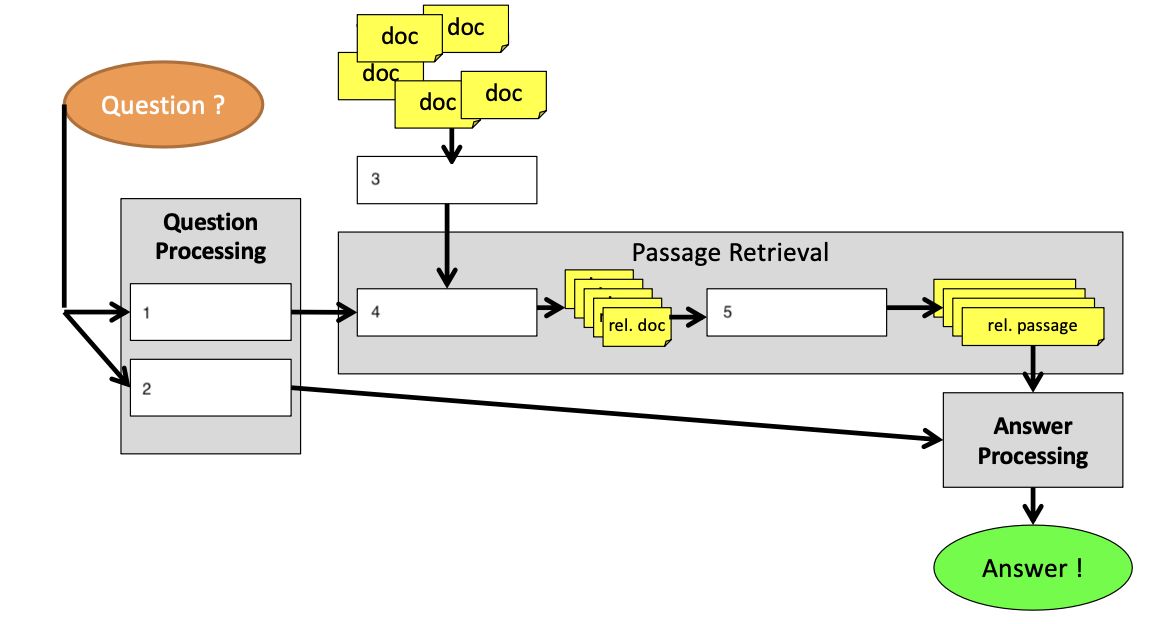
\includegraphics[width=.8\textwidth]{res/qa.png}
  \caption{Question Answering}\label{fig:qa}
\end{figure}

  Fill in the five white boxes in the image.

  \begin{solution}
    1. query formulation, 2. query classification, 3. indexing, 4. doc retrieval, 5. passage retrieval
  \end{solution}
\end{exercise}



\sheet[2021]{Exam}

\begin{exercise}{Comprehensiveness}
  What is comprehensiveness, specifically in the context of NLP?

  \begin{solution}
    Comprehensiveness refers to the extent to which a system, dataset, or model covers all relevant aspects of a task or domain.
    In NLP, comprehensiveness can be evaluated based on the coverage of linguistic phenomena, language varieties, or domain-specific terms in a dataset or model.
  \end{solution}
\end{exercise}

\begin{exercise}{Sequence tagging and CRF}\label{ex:seq-tagging}
  \begin{enumerate}
    \item What is sequence tagging in NLP?
    \item Explain the role of Conditional Random Fields (CRF) in sequence tagging.
  \end{enumerate}

  \begin{solution}
    \begin{enumerate}
        \item Sequence tagging assigns labels to each token in a sequence (e.g., POS tagging, named entity recognition).
        \item CRF is a probabilistic model that considers the dependencies between labels in a sequence, improving tagging accuracy by modeling label transitions.
    \end{enumerate}
  \end{solution}
\end{exercise}

\begin{exercise}{Feature differences}
  Explain the differences in features between classical ML and deep network-based ML.

  \begin{solution}
    \begin{itemize}
        \item \textbf{Classical ML} relies on manually engineered features (like tf-idf or n-grams) and requires domain expertise for feature extraction.
        \item \textbf{Deep networks} automatically learn hierarchical feature representations from raw data, capturing complex patterns and dependencies, but requiring large datasets for training.
    \end{itemize}
  \end{solution}
\end{exercise}

\begin{exercise}{Translate datasets}
  What are the pros and cons of translating datasets for NLP tasks? List 3 for each.

  \begin{solution}
    \begin{itemize}
        \item[+] Expands dataset availability to resource-scarce languages.
        \item[+] Enables cross-lingual NLP research.
        \item[+] Saves effort in recreating annotations.
        \item[-] Potential loss of annotation quality in translation.
        \item[-] Context or cultural relevance may not transfer.
        \item[-] Requires manual review to ensure correctness.
    \end{itemize}
  \end{solution}
\end{exercise}

\begin{exercise}{Pipeline}
  \begin{figure}
  \center
  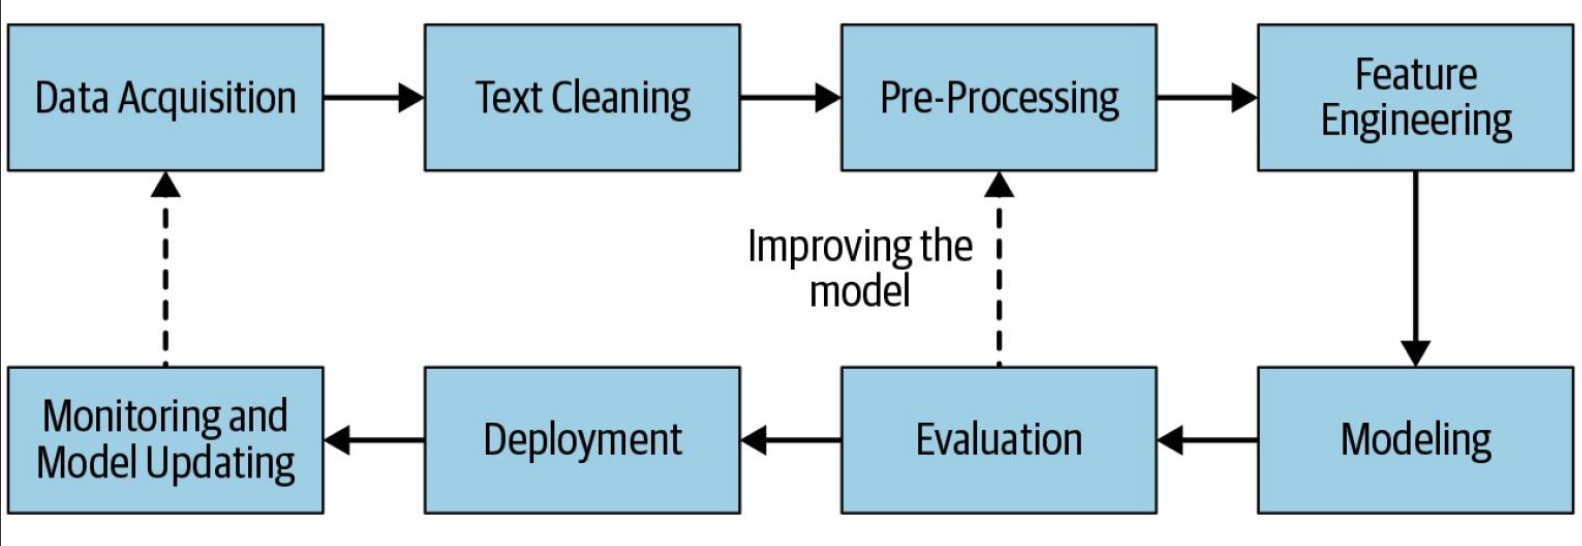
\includegraphics[width=.8\textwidth]{res/pipeline.png}
  \caption{NLP Pipeline}\label{fig:pipeline}
\end{figure}
  Assign three words to each stage of the given NLP pipeline in Figure \ref{fig:pipeline}.

  \begin{solution}
    \begin{itemize}
      \item \textbf{Data acquisition}: Crawling, scraping, downloading.
      \item \textbf{Text cleaning}: Tokenization, normalization, filtering.
      \item \textbf{Preprocessing}: Lemmatization, POS tagging, parsing.
      \item \textbf{Feature engineering}: TF-IDF, embeddings, n-grams.
      \item \textbf{Modeling}: Training, evaluation, and deployment.
      \item \textbf{Evaluation}: Metrics, analysis, feedback.
      \item \textbf{Deployment}: Integration, monitoring, maintenance.
      \item \textbf{Monitoring \& Model Updating}: Performance tracking, retraining, versioning.
    \end{itemize}
  \end{solution}
\end{exercise}

\begin{exercise}{MRR and accuracy}
  \begin{figure}
  \center
  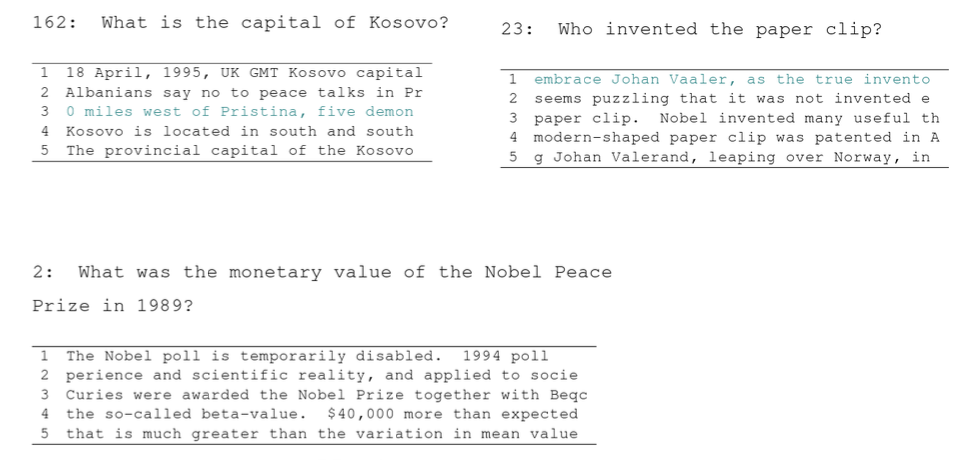
\includegraphics[width=.8\textwidth]{res/qa-answers.png}
  \caption{Question Answering}\label{fig:qa-answers}
\end{figure}
  Calculate Mean Reciprocal Rank (MRR) and Accuracy for the given query results in Figure \ref{fig:qa-answers} at $k=5$.

  \begin{solution}
    \begin{itemize}
        \item \textbf{Mean Reciprocal Rank} $MRR = \frac{1}{N} \sum_{i=1}^{N} \frac{1}{\text{rank}_i} = \frac{1}{3} (\frac{1}{3}+\frac{1}{1}+0 = .4444)$
        \item \textbf{Accuracy} $\frac{\text{Number of correct answers}}{\text{Total number of queries}} = \frac{2}{3} = .6666$
    \end{itemize}
  \end{solution}
\end{exercise}

\begin{exercise}{Spell checker}
  How does a spell checker handle non-words?

  \begin{solution}
    \begin{itemize}
        \item \textbf{Dictionary lookup}: Identify words not in the dictionary.
        \item \textbf{Edit distance}: Suggest corrections based on similarity (e.g., Levenshtein distance).
        \item \textbf{Contextual models}: Use surrounding words to predict the intended word.
    \end{itemize}
  \end{solution}
\end{exercise}

\begin{exercise}{Vector space}
  Explain Vector Space in Information Retrieval.

  \begin{solution}
    \begin{itemize}
        \item \textbf{Terms}: Each dimension corresponds to a term in the vocabulary.
        \item \textbf{Weights}: TF-IDF scores are used as weights for each term.
        \item \textbf{Similarity}: Compute cosine similarity to rank documents by relevance to the query.
    \end{itemize}
  \end{solution}
\end{exercise}

\begin{exercise}{Representation and fusion}
  What are representation and fusion in multimodal NLP, and how do they differ?

  \begin{solution}
    \begin{itemize}
        \item \textbf{Representation}: Encodes data (e.g., text or images) into feature vectors.
        \item \textbf{Fusion}: Combines multiple data modalities (e.g., text and images) to improve performance.
        \item \textbf{Differences}: Representation focuses on individual modalities, whereas fusion integrates multiple modalities into a unified representation.
    \end{itemize}
  \end{solution}
\end{exercise}

\begin{exercise}{Edit distance}\label{ex:edit-distance}
  \begin{enumerate}
    \item Define the Minimum Edit Distance.
    \item Calculate the Minimum Edit Distance for "TAC" vs. "CAT".
  \end{enumerate}

  \begin{solution}
    \begin{enumerate}
        \item The Minimum Edit Distance is the minimum number of operations (insertion, deletion, substitution) required to transform one string into another.
        \item The Minimum Edit Distance for "TAC" vs. "CAT" is 2.
    \end{enumerate}
  \end{solution}
\end{exercise}

\begin{exercise}{RAG and LangChain}\label{ex:rag}
  What is Retrieval-Augmented Generation (RAG), and how does LangChain assist in implementing it?

  \begin{solution}
    \begin{itemize}
        \item \textbf{RAG (Retrieval-Augmented Generation)}: Combines retrieval models with generative models to produce context-aware answers. External knowledge is retrieved and fed into the generation model.
        \item \textbf{LangChain}: A framework for building applications with large language models, offering tools for integrating RAG systems. It manages chaining retrieval and generation steps efficiently.
    \end{itemize}
  \end{solution}
\end{exercise}

\end{document}